
\documentclass[11pt]{article}
%\documentclass{book}
\usepackage[utf8]{inputenc}
\usepackage[T1]{fontenc}
\usepackage[french]{babel}
\usepackage[top=1.8cm, bottom=1.8cm, left=1.8cm, right=1.8cm]{geometry}
\usepackage[linktocpage,colorlinks=false]{hyperref}
\usepackage{graphicx}
\usepackage{epsfig}
\usepackage{amssymb}
\usepackage{amsmath}
\usepackage{array}
\usepackage{subfig}
\usepackage{multicol}
\usepackage{caption}
\usepackage{listings}
\usepackage{algorithm}
\usepackage{algorithmic}
\usepackage{enumitem}
\usepackage{titlesec}
\usepackage{array,multirow,makecell}
\hypersetup{
    colorlinks=true,
    breaklinks=true,
    urlcolor=red,
}
\parskip=5pt

\title{\huge{\textbf Compte Rendu \\  & \\  Outil automatique de décryptage (sujet 4)}}
\author{Chahi Rabie Ala Eddine, Arar Akram Mohamed, Attouche Maher, Benammar Ismail,\\ Chergou Amine Ismaïl, Ben Mallem Amir Fayçal, Mohammed Seghir Said, Yasmine Keskes.}
\date{Mardi 21 Mai 2019}


\begin{document}

\maketitle
    \vspace{20em}
    \begin{center}
\includegraphics[scale=0.50]{pictures/logo2.png}\end{center}
    \thispagestyle{empty}
\newpage

\tableofcontents
    \thispagestyle{empty}

\newpage
\setcounter{page}{1}
\section{Introduction}

La cryptologie est la science du secret des mathématiques et plus récemment de l’informatique, elle a permis le développement des échanges électroniques, tant dans le domaine industriel et bancaire que dans celui du commerce en ligne et récemment celui des relations entre les citoyens et les administrations. De ce fait un outil dédié à la cryptographie se veut d’une très grande utilité pour les chercheurs ou des personnes ayant de maigres connaissances dans le domaine et souhaitant apprendre davantage.

Dans le cadre du module \textit{Projet Informatique} du semestre 6 en licence à l’UVSQ, le sujet \textbf{Outil automatique de décryptage} nous a été attribué.
Ce projet a pour but de fournir une application qui permet d’interagir avec l’utilisateur à travers une interface graphique intuitive, afin de crypter, décrypter ou d’effectuer une cryptanalyse sur un texte soit par la méthode de Vigenère ou par substitution.

Après l’étude en détail des algorithmes de cryptographie et de la cryptanalyse dans le cahier des charges, et l'analyse de la mise en relation des différents modules correspondant aux différentes fonctionnalités, nous avons pu implémenter notre outil automatique de décryptage. Ce document va donc présenter le fonctionnement et l’architecture de l’application avec les explications techniques  sur les points délicats, ainsi qu’un bilan technique sur l’application et un bilan humain sur l’équipe de conception.

\section{Architecture de l'application}

\hspace{0.5cm}
\begin{center}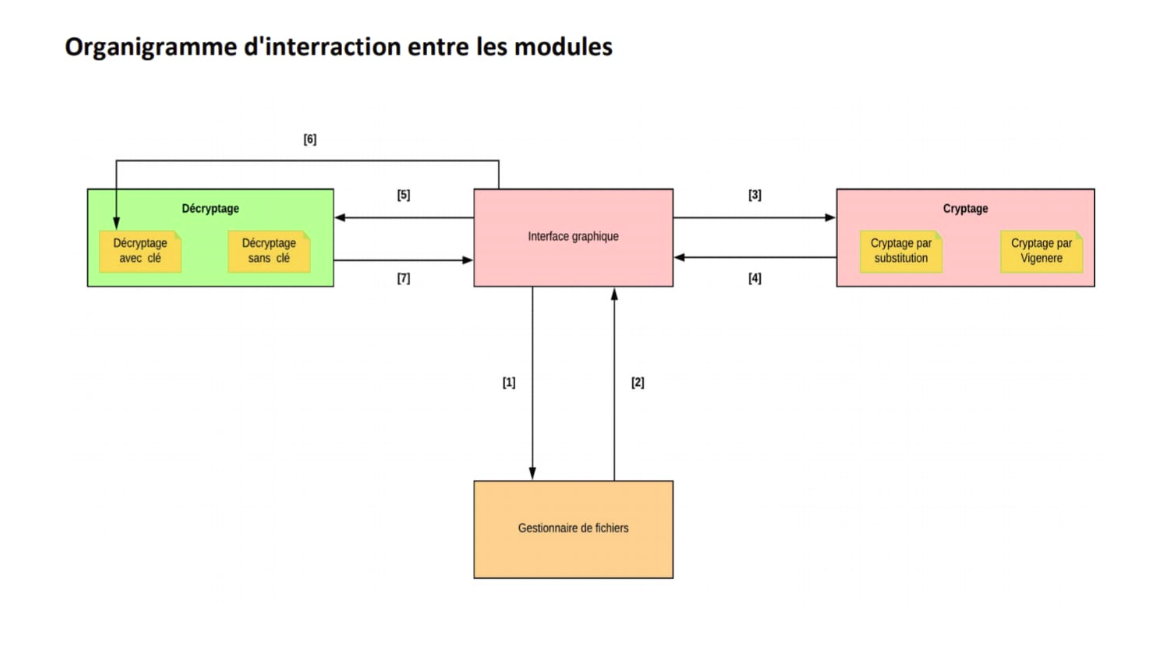
\includegraphics[scale=0.50]{pictures/Organigramme.png}\end{center}
\newpage
L'étude des algorithmes et des fonctionnalités et contraintes imposées par le client nous ont permis d'elaborer l'organigramme  ci-dessus qui présente l’architecture de l’application. Chaque module correspond à un ensemble de fonctionnalités assurant le bon fonctionnement de l’application. 



\textbf{L'outil comporte  4 modules:}
\begin{itemize}[label=\textbullet]
    \item Le module d'interface graphique gère l’interaction entre l'outil et l'utilisateur.
    \item Le module gestionnaire de fichiers assure les opérations de chargement et de sauvegarde de texte dans des fichier.
    \item Le module de cryptage assure le cryptage d'un texte donné en utilisant une clé de cryptage et ce soit par substitution ou selon la méthode de Vigenère.
    \item Le module de décryptage assure le décryptage d'un texte crypté auparavant soit par substitution soit par la méthode de Vigenère.
\end{itemize}
 L'utilisateur commence par introduire un texte ou bien sélectionner un fichier qui contient du texte pour charger ce dernier.
\\Si l'utilisateur désire charger un texte depuis un fichier, le chemin de celui-ci est envoyé vers le \textit{module gestionnaire de fichiers} (flèche 1) qui s'occupera de charger le texte et de le renvoyer vers le \textit{module Interface graphique} (flèche 2), après cela l'utilisateur peut soit crypter le texte soit le décrypter si ce dernier est déjà crypté.
Dans le cas où il désire crypter le texte, il devra saisir une clé et choisir le type du cryptage, ensuite le texte ainsi que la clé et la méthode choisie seront envoyés vers \textit{le module de cryptage} (flèche 3) qui se chargera de crypter le texte et de  renvoyer le résultat (flèche 4) vers \textit{le module interface graphique}.
Dans le cas contraire où l’utilisateur désire décrypter le texte, il devra renseigner la méthode  qui a servi pour crypter le texte  et éventuellement la clé qui a servi, si celle-ci est connue.
Dans le cas où la clé est connue elle est  envoyée depuis le module \textit{Interface graphique} au \textit{sous module décryptage avec clé} (flèche 6).
Le texte ainsi que le type de cryptage seront aussi envoyés depuis l’interface graphique vers le \textit{module décryptage} (flèche 5), qui se chargera de décrypter le texte et de renvoyer le résultat au \textit{module interface graphique} (flèche 7).
Au final si l’utilisateur désire exporter le texte vers un fichier, le texte ainsi que le chemin du fichier seront envoyés vers le \textit{module gestionnaire de fichiers} (flèche 1) qui se chargera de sauvegarder le texte dans le fichier.
\section{Prérequis}
Afin de garantir le bon fonctionnement de l'outil certaines règles doivent être réspectées :
\begin{itemize}[label=\textbullet]
   \item Les textes entrés afin de les crypter devront être écrit en langue française. 
   \item Les textes entrés afin de les cryptanalyser doivent être cryptés à partir d'un texte français correctement orthographié.
   \item Les textes très courts peuvent donner des résultats erronés lors de la cryptanalyse, pour cela il est préférable d'avoir un texte avec une longueur raisonnable. 
\end{itemize}
Remarque: Ceci est dû au fait que l'attaque statistique opère sur des textes suffisamment longs.

\section{Description du fonctionnement}

Dans cette partie nous allons mettre en évidence le fonctionnement interne de notre application. Pour cela, nous allons aborder avec précision chaque module de l’organigramme ainsi que les algorithmes implémentés. Enfin nous allons illustrer le fonctionnement de notre application par un exemple de déchiffrement d’un message sans clé. 

\subsection{Fonctionnement des modules}

\subsubsection{Interface graphique}

C'est le module qui s’occupe des interactions entre l’utilisateur et notre outil, en effet ce module offre à l’utilisateur la possibilité d’insérer ou de charger un texte et d’effectuer un des types de traitement que l’outil propose.
\subparagraph{Liste des fonctionalités}
\begin{itemize}[label=\textbullet]
    \item Choisir l’action à effectuer (Cryptage/Décryptage).
    \item Choisir le type de cryptage/décryptage (Substitution/Vigenère).
    \item Introduire un texte manuellement.
    \item Choisir un fichier source pour importer le texte Contenu dans le fichier.
    \item Choisir la clé avant de lancer le cryptage.
    \item Choisir de visualiser le déroulement du cryptage.
    \item Choisir de visualiser le déroulement du décryptage.
    \item Visualiser le texte en sortie.
    \item Choisir d’exporter le texte résultant vers un fichier.
\end{itemize}

\subsubsection{Cryptage}
Ce module assure le chiffrement d’un texte passé en paramètre en utilisant la méthode de Vigenère ou de substitution.

\paragraph{a) Cryptage par substitution :}
\newline
Ce sous module assure le cryptage d’un texte passé en paramètre avec une clé entrée par l’utilisateur ou générée aléatoirement.
\subparagraph{Liste des fonctionalités}
\begin{itemize}[label=\textbullet]
   \item Crypter un texte par substitution.
   \item Visualiser le déroulement du cryptage étape par étape.
\end{itemize}

\paragraph{b) Cryptage par Vigenère :}
\newline
Ce sous module assure le cryptage d’un texte passé en paramètre avec une clé entrée par l’utilisateur ou générée aléatoirement .
\subparagraph{Liste des fonctionalités}
\begin{itemize}[label=\textbullet]
   \item Crypter un texte par la méthode de blaise Vigenère.
   \item Visualiser le déroulement du cryptage étape par étape.
\end{itemize}
\subsubsection{Décryptage}
Ce module assure le décryptage d’un texte donné crypté auparavant soit par la méthode de substitution soit par la méthode de Vigenère.
\paragraph{a) Décryptage avec clé :}
\newline
Ce sous module assure le décryptage d’un texte donné en entrée et ce, en utilisant deux paramètres qui sont le type du cryptage ainsi que la clé utilisée lors du cryptage.
\newline Remarque : ce sous module trouve le texte résultant identique à 100\% au texte original.
\subparagraph{Liste des fonctionalités}
\begin{itemize}[label=\textbullet]
   \item Retrouver le texte original à partir d’un texte crypté par substitution et ce en utilisant une clé de décryptage.
   \item Retrouver le texte original à partir d’un texte crypté par la méthode de Vigenère et ce en utilisant une clé de décryptage.
   \item Visualiser le déroulement du décryptage étape par étape.
\end{itemize}
\paragraph{a) Décryptage sans clé :}
\newline
 Ce sous module assure le décryptage d’un texte donné en entrée à l'aide d'une attaque statistique, en utilisant un seul paramètre qui est le type du cryptage, ce sous module aide à
retrouver une grande partie du texte original à la différence du précédent qui a pour rôle
de retrouver 100\% du texte original.
\subparagraph{Liste des fonctionalités}
\begin{itemize}[label=\textbullet]
   \item Retrouver une grande partie du texte original à partir d’un texte crypté par substitution.
   \item Retrouver une grande partie du texte original à partir d’un texte crypté par la méthode de Vigenère.
   \item Visualiser le déroulement du décryptage étape par étape.
\end{itemize}

\subsubsection{Le module gestionnaire de fichiers}
Ce module permet de gérer du texte en entrée/sortie sur des fichiers, il offre la possibilité d’importer un texte clair ou chiffré contenu dans un fichier et de sauvegarder un texte résultant d’un des deux processus cryptage/décryptage dans un fichier.
\subparagraph{Liste des fonctionalités}
\begin{itemize}[label=\textbullet]
   \item Charger un texte depuis un fichier pdf/word/txt vers l’interface.
   \item Sauvegarder un texte affiché sur l’interface dans un fichier pdf/word/txt.
\end{itemize}

\subsection{Description des algorithmes proposés}

% mettre un prerequis disant que soit cest XOR soit cest pur melange

\subsubsection{Chiffrement par substitution mono-alphabétique }
Cet algorithme chiffre le texte clair modifié au préalable (sans espaces et le tout en majuscules), il prend en entrée la clé de taille 26, il effectue des permutations de sorte que chaque lettre de l’alphabet est remplacée par
la lettre qui correspond à son rang dans la clé.
\subparagraph{Exemple:}
\subsubparagraph{On souhaite chiffrer le mot "Exemple" en utilisant la clé
AZERTYUIOPQSDFGHJKLMWXCVBN .
\begin{itemize}[label=\textbullet]
\item On fait correspondre la clé de taille 26 au 26 lettes de l’alphabet : \\
AZERTYUIOPQSDFGHJKLMWXCVBN\\
ABCDEFGHIJKLMNOPQRSTUVWXYZ\\
\item Cela veut dire que tous les A dans le clair seront transformés en A dans le chiffré, tous les B en Z, les C en E .....etc.
Donc le mot Exemple est chiffré en "TVTDHST" .}
\end{itemize}
\subsubsection{Chiffrement par Vigenère}

Cet  algorithme chiffre le texte clair modifié au préalable (sans espaces et le tout en majuscules), il prend en paramètre une clé qu’il répète tout au long du texte et effectue une addition modulo 26 entre l’indice dans l’alphabet  de chaque lettre de la clé avec la lettre  du texte qui lui correspond.

\subparagraph{Exemple}: 
On souhaite chiffrer le mot "Exemple" en utilisant la clé "KEY" :\\
\begin{itemize}[label=\textbullet]
\item On commence par répéter la clé tout le long du texte. 
\item Afin de trouver le chiffré on fait l'addition modulo 26 du rang de la lettre du clair avec le rang de la lettre de la clé.\\
Clair :   \ \ \ \ \  EXEMPLE \ \ \ \ \  [4 23 4 12 15 11 4] \\ 
Clé : \  \ \ \ \ \ \ KEYKEYK \ \ \ \  [10 4 23 10 4 23 10] \\
Resultat : OBCWTJO. \ \ \ \  [14 1 2 22 19 9 14]
\end{itemize}

\subsubsection{Déchiffrement par substitutions mono-alphabétique}
Cet algorithme prend en entrée une clé de taille 26 qui contient les permutations des lettres de l’alphabet, exemple : on permute A par D donc à l’indice zéro qui correspond au rang de la lettre A dans l’alphabet on trouve la lettre D.
Pour chaque lettre du texte chiffré on parcourt la clé dès qu’on trouve la lettre en question on prend son indice dans la clé pour retrouver le clair de cette lettre il suffit de voir la lettre qui correspond à cet indice dans l’alphabet. 
\subparagraph{Exemple:}
\subsubparagraph{On souhaite déchiffrer le mot "TVTDHST" en utilisant la clé \\
AZERTYUIOPQSDFGHJKLMWXCVBN .
\begin{itemize}[label=\textbullet]
\item On fait correspondre la clé de taille 26 au 26 lettes de l’alphabet : \\
AZERTYUIOPQSDFGHJKLMWXCVBN\\
ABCDEFGHIJKLMNOPQRSTUVWXYZ\\
\item Cela veut dire que tous les A dans le chiffré seront transformés en A dans le clair, tous les Z en B, les E en C .....etc.
Donc le mot TVTDHST est déchiffré en "EXEMPLE" .}
\end{itemize}
\subsubsection{Déchiffrement de Vigenère}
Cet algorithme permet de déchiffrer un texte chiffré à l’aide de la clé passée en paramètre, il découpe le texte en blocs qui font la même taille que la clé, puis il  correspond chaque bloc crypté à la clé et soustrait le rang (dans l’alphabet) de la lettre de la clé  du rang de la lettre du texte chiffré le tout modulo 26.
\subparagraph{Exemple}: 
On souhaite déchiffrer le mot "OBCWTJO" en utilisant la clé "KEY" :\\
\begin{itemize}[label=\textbullet]
\item On commence par répéter la clé tout le long du texte. 
\item Afin de trouver le clair on fait la soustraction modulo 26 du rang de la lettre du chiffré avec le rang de la lettre de la clé.\\ \newpage
Chiffré :   \ \ \  OBCWTJO \ \ \ \ \  [14 1 2 22 19 9 14] \\ 
Clé : \  \ \ \ \ \ \ \ KEYKEYK \ \ \ \  [10 4 23 10 4 23 10] \\
Resultat :  \ EXEMPLE. \ \ \ \  [4 23 4 12 15 11 4]
\end{itemize}



\subsubsection{Algorithme d’analyse des fréquences}
Cet algorithme prend en entrée un texte chiffré, et remplit la structure de données qui est une table de hachage, contenant les lettres de l’alphabet, les digrammes et les trigrammes avec leurs fréquences et positions dans le texte.

\subsubsection{Algorithme de cryptanalyse de la substitution monoalphabétique}
Cet algorithme a pour rôle de trouver une grande partie du texte chiffré sans la clé, dans un premier
temps on génére une clé aléatoire puis on déchiffre le texte à l’aide de cette clé, une fois le texte déchiffré on le divise en quadrigrammes et on calcule le taux de compatibilité entre les fréquences des quadrigrammes dans le déchiffré et ceux de la langue française, on garde la permutation de la clé et son taux de compatibilité, ensuite on refait le même procédé en permutant les lettres de la clé si on trouve un taux de compatibilité meilleur par rapport à l’ancien on remplace l’ancienne permutation par la nouvelle permutation. Dans le cas où le taux de compatibilité ne change pas au bout de plusieurs itérations alors la permutation de la clé est probablement la bonne. \\
\textbf{Remarque}: dans cette algorithme on a utilisé les 30 000 quadrigrammes les plus fréquents dans la langue française.
\subparagraph{Exemple:} 
On possède un texte chiffré par substitution que l'on souhaite cryptanalyser :\\
"XOUENFTZOUXFZFBLAHAIEJACJF" \\
\begin{itemize}[label=\textbullet]
   \item On commence par choisir une clé aléatoire de taille 26 : \\
\ \ \ \ BDCSFGMPILKJHNORQZETUXWVAY   
   \item On déchiffre le texte en utilisant cette clé ce qui nous donne \\
VOUSNETROUVEREAJYMYISLYCLE.
\item On calcule le taux de compatibilité du texte déchiffré \\
 \[ Taux = \frac{Prob(VOUS) + Prob(OUSN) + Prob(USNE) + Prob(SNET)......… }{n} \]
 \ \ \ \ avec n le nombre de quadrigrammes dans le texte.
\item On Fait des permutations dans la clé afin d'améliorer le taux \\
Si on permute le A avec le Y , le résultat du déchiffrement sera : \\
VOUSNETROUVEREZJAMAISLACLE \\
On remarque que le texte est plus lisible et son taux de compatibilité est meilleur donc on garde cette nouvelle clé. \\
\item  On essaye de trouver une permutation qui améliore le taux mais au bout de plusieurs tests aucune permutation n'améliore le taux donc on garde cette clé.
\end{itemize}

 \subsection{Algorithme de cryptanalyse de Vigenère }
 Cet algorithme a pour rôle de retrouver une grande partie du texte original à partir d'un texte crypté, en premier lieu cet algorithme commence par trouver la longueur de la clé qui a servi lors du cryptage et ce en utilisant l'algorithme de Kasiski expliqué ci-desous.
 
 \subsection{Algorithme de Kasiski}
 Afin de trouver la longueur de la clé, l'algorithme commence par trouver les polygrammes fréquents dans le texte, il calcule ensuite les distances qui séparent chaque occurrence du même polygramme ainsi que les diviseurs de ces distances.
De cette manière le diviseur le plus commun entre les différents polygrammes et probablement la longueur de la clé.

\subsubsection{Algorithme de l’indice de coïncidence}
 Pour confirmer que la longueur (n) de la clé trouvée est bien celle utilisée pour crypter le texte, le texte est divisé en n parties de sorte que chaque partie est supposée être cryptée en utilisant le même caractère de la clé, ensuite l'indice de coïncidence de chaque partie est calculé.\\
Si l'indice est proche de 0.0735 qui est l'indice de coïncidence moyen d'un texte écrit en français alors la longueur trouvée est bien celle qui a servi pour crypter le texte.\\ Sinon le même processus est refait pour les autres longueurs probables. \\
Après avoir trouvé la longueur n de la clé, l'algorithme découpe le texte en n parties. Dans ce cas chaque partie (Li) a été cryptée en utilisant la lettre i de la clé.
Afin de retrouver la i ème lettre de la clé, une attaque statistique est utilisée sur la partie (Li).

\subsubsection{Algorithme de l’attaque statistique}
Afin de retrouver la lettre (décalage) i qui a servi à crypter un texte, une analyse est faite sur le texte pour retrouver le caractère le plus fréquent, ce caractère représente forcément le caractère E de l’alphabet crypté en utilisant le décalage i.
donc afin de retrouver le décalage i, il suffit de soustraire le rang de E (4) du rang du caractère le plus fréquent.\\
Une fois la clé retrouvée il suffit de décrypter le texte en utilisant cette dernière.
\subparagraph{Exemple d'algorithme de cryptanalyse de Vigenère en utilisant l’algorithme de Kasiski, Indice de coïncidence ainsi que l’algorithme de l’attaque statistique : } \ \ \ \ \ \ \ \ \ \ \ \ \ \ \ \ \ \ \ \ \ \ \ \ \ \ \ \ \ \ \ \ \ \ \ \ \ \ \ \ \ \ \ \ \ \ \ \ 

On possède un texte chiffré par Vigenère que l'on souhaite cryptanalyser : \\
"WIQCEEOVRBIQWIQAYGXQCCSNYVRKML" \\
\begin{enumerate}
\item On commence par rechercher les polygrammes les plus fréquents. \\
On trouve que le Trigramme(WIQ), Bigramme(IQ), Bigramme(VR) sont fréquents et se répètent  plusieurs fois. \\
\item On calcule les distances qui séparent chaque répétition du même polygramme. \\
WIQ : 12 \\
IQ : 9 , 12 \\
VR : 18 \\
\item On calcule ensuite les diviseurs de chaque groupe de distances. \\
Diviseurs (WIQ): 1,2,3,4,6 \\
Diviseurs (IQ): 1,3,6,9,12 \\
Diviseurs (VR): 1,2,3,6,9 \\
\item On trouve que les diviseurs les plus fréquents sont 6 et 3. Donc la clé est probablement de longueur 3 ou 6 \\
\item On essaye Longeur=3. \\
\item On divise le text chiffré en 3 groupes : \\
g1 g2 g3 \\  
W  I  Q \ \ \ \ \ \ - Tous les éléments du groupe g1 ont été crypté en utilisant la même partie de la clé. \\   
C  E  E	\\
O  V  R \ \ \ \ \ \ - On Trouve que l'élément le plus répété dans le g1 est O qui correspond forcément au E. \\   
B  I  Q	\\
W  I  Q \ \ \ \ \ \ - On calcule alors la 1ére lettre de la clé O-E=K. \\
A  Y  G	 \\
X  Q  C \ \ \ \ \ \ - On fait de même pour les deux groupes g2 et g3.\\	 
O  S  N \\
Y  V  R \ \ \ \ \ \ - On trouve la clé = KEY. \\
K  M  L \\
\item On décrypte le texte en utilisant la clé KEY \\
on trouve "MESSAGERTRESMEQUINMESOPORTAIN".
\end{itemize}
 
\subsection{Fonctionnement de l'outil par un exemple de cryptanalyse par Vigenère}

Un utilisateur choisit de déchiffrer un message crypté par la méthode de Vigenère sans avoir la clé, il a le choix entre, entrer le texte via l'interface graphique ou bien de le charger depuis un fichier, on suppose que le texte est entré via l’interface, ceci aura pour effet d’initialiser un objet de type polygramme qui se chargera de calculer les fréquences des lettres, digrammes, trigrammes ainsi que des quadrigrammes et récupérer leurs positions dans le texte puis stocke les informations de ces derniers successivement dans les structures de données suivantes  \textit{map<string,Polygramme *> bigram, map<string,Polygramme *> trigram, map<string,Polygramme *> quadrigram}.
La méthode  \textit{TextV::findKeySize()} qui est une implémentation de l’algorithme de Kasiski sera appelée pour trouver la taille de la clé utilisée ceci en calculant les distances entre les différents polygrammes, puis trouve les diviseurs de ces distances et cherche le diviseur commun le plus répété qui sera probablement la taille de la clé la taille de la clé sera confirmé grâce à l’indice de coïncidence.
Une fois la taille de la clé retrouvée on fait appel à la méthode \textit{TextV::findKeyUsed(KeySize)} qui prend en paramètre la taille de la clé, elle aura pour rôle de retrouver la clé utilisée et cela en faisant une attaque statistique c’est-à-dire, on effectue une analyse fréquentielle sur  l’alphabet L1 qui correspond à l’ensemble des lettres du texte chiffré à partir de la première lettre de la clé afin d’obtenir cette dernière et on réitère l’opération sur L2 jusqu’à Ln ou n correspond la taille de la clé . 
Une fois la clé retrouvée il nous reste plus qu’à déchiffrer le texte, et ce en utilisant la méthode  \textit{TextV::decrypt(Key)} qui prend en paramètre la clé, cette méthode effectue une soustraction modulo 26 entre l’indice dans l’alphabet de chaque lettre du texte avec l’indice de l’alphabet de la lettre de la clé qui lui correspond.

\section{Choix du language de programmation :}
Nous avons opté pour le \textit{C++} car c'est un langage hybride offrant la possibilité d’utiliser l’aspect procédural afin de gérer tout ce qui touche aux routines mathématiques calculatoires qui sont le pilier de notre projet, ainsi que la gestion de fichiers. \\
Le \textbf{C++} offre aussi la possibilité d'utiliser l’aspect orienté objet, en effet, tout dans notre projet peut être vu comme étant un objet, que ce soit un texte, un polygramme ou bien même une clé de cryptage ou de décryptage, nous avons également eu besoin de la notion d'héritage afin de pouvoir implémenter notre code d'une façon optimal, ainsi nous avons par exemple pu faire hériter deux différents types de texte d'une classe mère (Text) et qui sont, TextV (Vigenère) et TextS (Substitution) qui ont chacune des méthodes propres à elles-mêmes.
De plus, nous avons aussi eu besoin  de les notions de polymorphisme et de surcharge, en effet la méthode de décryptage diffère selon la présence ou non d'une clé de décryptage et selon le type du texte à décrypter (Substitution ou bien Vigenère).
Nous avons aussi eu besoin de l'aspect orienté objet dans le but de modulariser le code, de l’aérer et d’en faciliter la modification.

Choix du Framework \textbf{Qt}: \\
Qt possède une documentation assez complète qui explique le fonctionnement de certaines classes en détail ce qui nous a été grandement utile lors de l'implémentation de notre interface graphique. Le framework \textbf{Qt} possède un ensemble de bibliothèques permettant de développer des application complexe.

Enfin nous avons à disposition un ensemble d’outils facilitant le développement d’applications. Il faut savoir que comme le framework fonctionne sur les trois systèmes d’exploitation (Mac OS, Linux et Windows), ces outils sont eux aussi compatibles avec l’ensemble des systèmes.


\section{Description des points délicats de la programmation}
\begin{itemize}[label=\textbullet]
\item Lors de l’implémentation de la cryptanalyse par substitution nous avons rencontré un problème qui n’était pas évident à détecter, en effet lorsqu’on rencontrait des quadrigrammes avec une fréquence nul dans la langue française cela avait pour effet de mettre le taux de compatibilité à moins l’infinie cela est dû à l’utilisation de la fonction logarithme, afin de remédier à ce problème nous avons dû donner une fréquence très faible pour l’ensemble
des quadrigrammes ayant la fréquence nul.
\item Lors de l'implementation de la cryptanalyse par substitution nous avons remarqué que lorsqu'on générait une première clé totalement aléatoire, l'exécution de l'algorithme prenait du temps, afin de remédier à ce problème et d'optimiser le temps d'exécution nous avons opté pour la génération d'une première clé par le biais d'une attaque statistique sur le texte, celle-ci étant très proche de la clé effective elle diminue considérablement le temps d'exécution.
\item Lors de la réalisation du déroulement de la cryptanalyse de Vigenère on a eu des difficultés à récupérer quelques informations nécessaires au bon fonctionnement du déroulement des
différentes étapes du décryptage sans clé, afin de remédier à ce problème nous avons décidé d’envoyer ces informations depuis la méthode decrypt() vers la méthode responsable du déroulement.
\end{itemize}
\section{Comparaison entre l'estimation et l'implémentation}

\small
\hspace{-2cm}
\begin{tabular}{|c|c|c|c|}
  \hline
  \textbf{Module de l'application} & \textbf{Coût en temps} & \textbf{Coût en nombre de lignes} & \textbf{Personnes en charge} \\
  \hline
    Interface & Estimation : 18 heures & Estimation :800 lignes & Atouche Maher \& \\ 
    graphique & Implémentation : 16 heures & Implémentation :732 lignes & Chahi Rabie Ala Eddine \\
  \hline
    Cryptage et décryptage & Estimation : 6 heures & Estimation :100 lignes & Mohammed Seghir Said \& \\
  par substitution & Implémentation : 2 heure & Implémentation : 65 lignes  & Yasmine Keskes \\
  \hline
  Cryptage et décryptage & Estimation : 6 heures & Estimation : 100 lignes & Amir Fayçal Ben Mallem  \& \\
   par Vigenère & Implémentation : 2 heures & Implémentation : 15 lignes & Benammar Ismail \\
  \hline
    Géstionnaire de & Estimation : 12 heures & Estimation : 200 lignes & Arar Akram Mohamed \& \\
   de fichiers & Implémentation : 12 heures & Implémentation :160 lignes & Chergou Amine Ismaïl \\
  \hline
    Cryptanalyse par & Estimation : 75 heures & Estimation : 350 lignes &  Benammar Ismail \&  Yasmine Keskes  \\
   substitution & Implémentation : 50 heures & Implémentation : 140 lignes & \& Amir Fayçal Ben Mallem \\
    \hline
    Cryptanalyse de & Estimation : 65 heures & Estimation : 250 lignes & Chergou Amine \&  Mohammed Seghir  \\
   Vigenère & Implémentation : 35 heures & Implémentation : 280 lignes & \& Arar Akram Mohamed \\
   \hline
    Déroulement des & Estimation : 36 heures & Estimation : 800 lignes & Attouche Maher  \\
   étapes crptage/décryptage & Implémentation : 28 heures & Implémentation : 800 lignes & \& Chahi Rabie Ala Eddine \\
  \hline
    & & &  \\
   Le coût  & Estimation :182  heures & Estimation : 2600 lignes & \\
   total & Implémentation : 145 heures & Implémentation : 2192 lignes &  \\  
  \hline
\end{tabular}
\normalsize
\vspace{0.5cm}

On peut remarquer dans certains cas des différences plus ou moins grandes entre les estimations en nombre de lignes et d'heures de travail et le coût réel et ce pour des raisons différentes :
\begin{itemize}[label=\textbullet]
\item Dans le cas du cryptage/décryptage avec clé que ce soit par substitution ou selon la méthode de Vigenère, on peut remarquer que le travail a été plus court que prévu, cela est dû au fait que nous avions prévu un temps pour la documentation, mais vu que durant ce semestre nous avons eu une UE de Cryptographie où on a traité ces différentes méthodes de cryptage/décryptage le travail de recherche a été minime.  
\item Dans le cas de la cryptanalyse de Vigenère et Substitution, on peut remarquer qu'il y a une différence entre le taux horaire estimé et celui réel, ceci peut être expliqué par le fait que nous avions estimé que le taux d'erreur initial serait un peu élevé et que nous aurions à l'améliorer au cours du temps, chose qui a été faite plus rapidement que prévu. 

\end{itemize}

\section{Conclusion technique}
Notre outil satisfait actuellement la totalité des objectifs fixés par le client, en plus de ces objectifs notre outil répond également à certaines éxigences supplémentaire motivées pour certaines par le client, d'autres par nous-même en guise de geste commercial. \\
En effet notre outil est capable de crypter/décrypter un texte soit par substitution ou selon la méthode de Vigenère et ce avec ou sans clé le tout via une interface graphique ergonomique et facile d'accès, en plus l'équipe Cryptopher s'est investi afin de réaliser les fonctionnalités supplémentaires demandées par le client lors des réunions, tel que l'affichage dynamique des étapes de déroulement des cryptage/décryptage/cryptanalyse ainsi que le chargement et l'exportation de texte depuis et dans des fichiers de différents formats tels que txt,word,pdf. \\
Cependant l'équipe n'a pas eu le temps de finir le déroulement de la cryptanalyse par substitution, cette fonctionnalité étant presque prête elle sera finalisée avant le 28/05/2019.

Lors de la conception l'équipe a veillé à ce que l'outil soit parfaitement modulaire afin de faciliter la modification et l'ajout de fonctionnalités.
En effet certaines perspectives d'améliorations sont envisagées, tels que l'ajout de nouveaux types de chiffrement tel que Enigma,Hill,ElGamal... etc.
L'ajout de la langue anglaise est aussi envisageable.
\section{Conclusion sur l'organisation interne au sein du projet}
Durant 16 semaines, notre équipe s’est surpassé afin de réaliser le projet du module IN608 intitulé \textit{outil automatique de décryptage}, ce projet fut l’occasion pour les membres de l’équipe de mettre à profit les acquis et les bonnes pratiques accumulées durant nos trois années de licence, en effet dès la première réunion tout le monde était d’accord pour dire que l’organisation serait la clé de voûte du succès de notre projet, pour cela, il nous tenait à cœur de réaliser un outil qui satisfait la totalité des exigences du client, et ce, en élaborant des plannings qui ont toujours été respectés, ainsi qu’une répartition équitable des tâches.
Nous avons décidé de désigner un chef de projet qui avait pour rôle de veiller à ce que le travail soit effectué en respectant les délais mais aussi le maintien d’une bonne entente et communication au sein du groupe.
Au final le projet s’est avéré être un point indispensable dans notre apprentissage ainsi qu’une excellente première expérience de travail dans une grande équipe, la réalisation de cet outil nous a beaucoup apporté tant sur le plan professionnel que sur le plan humain.
\end{document}
